\documentclass{article}

\usepackage{imports}
\usepackage{pgfplots}
\usepackage{tikz}

\pgfplotsset{compat=1.16}

\begin{document}


%%%%%%%%%%%%%%%%%%%%%%%%%%%%%%%%%%%%%%%%%%%%%%%%%%%%%%%%%%%%%%%%%%%%%%%%%%%%%%%%%%%%%%
%%%%%%%%%%%%%%%%%%%%%%%%%%%%%%%%%%%%%%%%%%%%%%%%%%%%%%%%%%%%%%%%%%%%%%%%%%%%%%%%%%%%%%
%%%%%%%%%%%%%%%%%%%%%%%%%%%%%%%%%%%%%%%%%%%%%%%%%%%%%%%%%%%%%%%%%%%%%%%%%%%%%%%%%%%%%%

\section*{Monotone, Linear, Rank Similar, No Heterogeneity:}

%%%%%%%%%%%%%%%%%%%%%%%%%%%%%%%%%%%%%%%%%%%%%%%%%%%%%%%%%%%%%%%%%%%%%%%%%%%%%%%%%%%%%%
%%%%%%%%%%%%%%%%%%%%%%%%%%%%%%%%%%%%%%%%%%%%%%%%%%%%%%%%%%%%%%%%%%%%%%%%%%%%%%%%%%%%%%

\begin{align*}
    ValueAdded = TeacherAbility
\end{align*}

\begin{tikzpicture}
    \begin{axis}[ymin=0.25, ymax=0.75, ytick={0.5}, yticklabel=$TeacherAbility$, axis x line=bottom, axis y line=left, xlabel = Student Ability Percentile]
        \addplot[domain=0:1, blue, ultra thick] {0.5};
    \end{axis}
\end{tikzpicture}




%%%%%%%%%%%%%%%%%%%%%%%%%%%%%%%%%%%%%%%%%%%%%%%%%%%%%%%%%%%%%%%%%%%%%%%%%%%%%%%%%%%%%%
%%%%%%%%%%%%%%%%%%%%%%%%%%%%%%%%%%%%%%%%%%%%%%%%%%%%%%%%%%%%%%%%%%%%%%%%%%%%%%%%%%%%%%
%%%%%%%%%%%%%%%%%%%%%%%%%%%%%%%%%%%%%%%%%%%%%%%%%%%%%%%%%%%%%%%%%%%%%%%%%%%%%%%%%%%%%%

\section*{Monotone, Linear, Rank Similar:}

%%%%%%%%%%%%%%%%%%%%%%%%%%%%%%%%%%%%%%%%%%%%%%%%%%%%%%%%%%%%%%%%%%%%%%%%%%%%%%%%%%%%%%
%%%%%%%%%%%%%%%%%%%%%%%%%%%%%%%%%%%%%%%%%%%%%%%%%%%%%%%%%%%%%%%%%%%%%%%%%%%%%%%%%%%%%%

\begin{align*}
    ValueAdded = TeacherAbility + MaxDifference*StudentPercentile - \frac{1}{2}MaxDifference
\end{align*}

\begin{tikzpicture}
    \begin{axis}[ymin=0.25, ymax=0.75, ytick={0.5}, yticklabel=$TeacherAbility$, axis x line=bottom, axis y line=left, xlabel = Student Ability Percentile]
        \addplot[domain=0:1, blue, ultra thick] {0.1*x + .45};
        \addplot[domain=0:1, mark=-, red, dashed] {0.5};
    \end{axis}
\end{tikzpicture}




%%%%%%%%%%%%%%%%%%%%%%%%%%%%%%%%%%%%%%%%%%%%%%%%%%%%%%%%%%%%%%%%%%%%%%%%%%%%%%%%%%%%%%
%%%%%%%%%%%%%%%%%%%%%%%%%%%%%%%%%%%%%%%%%%%%%%%%%%%%%%%%%%%%%%%%%%%%%%%%%%%%%%%%%%%%%%
%%%%%%%%%%%%%%%%%%%%%%%%%%%%%%%%%%%%%%%%%%%%%%%%%%%%%%%%%%%%%%%%%%%%%%%%%%%%%%%%%%%%%%

\section*{Monotone, Linear:}

%%%%%%%%%%%%%%%%%%%%%%%%%%%%%%%%%%%%%%%%%%%%%%%%%%%%%%%%%%%%%%%%%%%%%%%%%%%%%%%%%%%%%%
%%%%%%%%%%%%%%%%%%%%%%%%%%%%%%%%%%%%%%%%%%%%%%%%%%%%%%%%%%%%%%%%%%%%%%%%%%%%%%%%%%%%%%

\begin{align*}
    ValueAdded = TeacherAbility - MaxDifference*StudentPercentile + \frac{1}{2}MaxDifference
\end{align*}

\begin{tikzpicture}
    \begin{axis}[ymin=0.25, ymax=0.75, ytick={0.5}, yticklabel=$TeacherAbility$, axis x line=bottom, axis y line=left, xlabel = Student Ability Percentile]
        \addplot[domain=0:1, blue, ultra thick] {-0.1*x+0.55};
        \addplot[domain=0:1, mark=-, red, dashed] {0.5};
    \end{axis}
\end{tikzpicture}




%%%%%%%%%%%%%%%%%%%%%%%%%%%%%%%%%%%%%%%%%%%%%%%%%%%%%%%%%%%%%%%%%%%%%%%%%%%%%%%%%%%%%%
%%%%%%%%%%%%%%%%%%%%%%%%%%%%%%%%%%%%%%%%%%%%%%%%%%%%%%%%%%%%%%%%%%%%%%%%%%%%%%%%%%%%%%
%%%%%%%%%%%%%%%%%%%%%%%%%%%%%%%%%%%%%%%%%%%%%%%%%%%%%%%%%%%%%%%%%%%%%%%%%%%%%%%%%%%%%%

\section*{Monotone, Non-linear, Rank Similar:}

%%%%%%%%%%%%%%%%%%%%%%%%%%%%%%%%%%%%%%%%%%%%%%%%%%%%%%%%%%%%%%%%%%%%%%%%%%%%%%%%%%%%%%
%%%%%%%%%%%%%%%%%%%%%%%%%%%%%%%%%%%%%%%%%%%%%%%%%%%%%%%%%%%%%%%%%%%%%%%%%%%%%%%%%%%%%%

\begin{align*}
    ValueAdded = & TeacherAbility + Height*MaxDifference*StudentPercentile^{ExpNum} \\ 
    & - \frac{Height*MaxDifference}{ExpNum + 1}
\end{align*}

\begin{tikzpicture}
    \begin{axis}[ymin=0.25, ymax=0.75, ytick={0.5}, yticklabel=$TeacherAbility$, axis x line=bottom, axis y line=left, xlabel = Student Ability Percentile]
        \addplot[domain=0:1, blue, ultra thick] {.1*(x)^5 + .5 - .1/6};
        \addplot[domain=0:1, mark=-, red, dashed] {0.5};
    \end{axis}
\end{tikzpicture}


%%%%%%%%%%%%%%%%%%%%%%%%%%%%%%%%%%%%%%%%%%%%%%%%%%%%%%%%%%%%%%%%%%%%%%%%%%%%%%%%%%%%%%
%%%%%%%%%%%%%%%%%%%%%%%%%%%%%%%%%%%%%%%%%%%%%%%%%%%%%%%%%%%%%%%%%%%%%%%%%%%%%%%%%%%%%%

\begin{align*}
    ValueAdded = & TeacherAbility \\
    & + \mathbbm{1}(StudentPercentile < Jump1)*Height*MaxDifference*StudentPercentile^{ExpNum} \\ 
    & + \mathbbm{1}(StudentPercentile >= Jump1)*Height*MaxDifference \\
    & - \frac{Jump1*Height*MaxDifference}{ExpNum + 1} - (1 - Jump1)*Height*MaxDifference
\end{align*}

\begin{tikzpicture}
    \begin{axis}[ymin=0.25, ymax=0.75, ytick={0.5}, yticklabel=$TeacherAbility$, axis x line=bottom, axis y line=left, xlabel = Student Ability Percentile]
        \addplot[domain=0:0.5, blue, ultra thick] {.1*((1/0.5)*x)^5 + .5 - (.1*.5)/6 - .5*.1};
        \addplot[domain=0.5:1, blue, ultra thick] {.6 - (.1*.5)/6 - .5*.1};
        \addplot[domain=0:1, mark=-, red, dashed] {0.5};
    \end{axis}
\end{tikzpicture}


%%%%%%%%%%%%%%%%%%%%%%%%%%%%%%%%%%%%%%%%%%%%%%%%%%%%%%%%%%%%%%%%%%%%%%%%%%%%%%%%%%%%%%
%%%%%%%%%%%%%%%%%%%%%%%%%%%%%%%%%%%%%%%%%%%%%%%%%%%%%%%%%%%%%%%%%%%%%%%%%%%%%%%%%%%%%%

\begin{align*}
    ValueAdded = & TeacherAbility + \mathbbm{1}(StudentPercentile >= Jump1)*DiffSize*MaxDifference \\
    & - (1 - Jump1)*DiffSize*MaxDifference
\end{align*}

\begin{tikzpicture}
    \begin{axis}[ymin=0.25, ymax=0.75, ytick={0.5}, yticklabel=$TeacherAbility$, axis x line=bottom, axis y line=left, xlabel = Student Ability Percentile]
        \addplot[domain=0:.5, blue, ultra thick] {.5 - (.5*.1)};
        \addplot[domain=.5:1, blue, ultra thick] {.5 + .1 - (.5*.1)};
        \addplot[domain=0:1, mark=-, red, dashed] {0.5};
    \end{axis}
\end{tikzpicture}




%%%%%%%%%%%%%%%%%%%%%%%%%%%%%%%%%%%%%%%%%%%%%%%%%%%%%%%%%%%%%%%%%%%%%%%%%%%%%%%%%%%%%%
%%%%%%%%%%%%%%%%%%%%%%%%%%%%%%%%%%%%%%%%%%%%%%%%%%%%%%%%%%%%%%%%%%%%%%%%%%%%%%%%%%%%%%
%%%%%%%%%%%%%%%%%%%%%%%%%%%%%%%%%%%%%%%%%%%%%%%%%%%%%%%%%%%%%%%%%%%%%%%%%%%%%%%%%%%%%%

\section*{Monotone, Non-linear:}

%%%%%%%%%%%%%%%%%%%%%%%%%%%%%%%%%%%%%%%%%%%%%%%%%%%%%%%%%%%%%%%%%%%%%%%%%%%%%%%%%%%%%%
%%%%%%%%%%%%%%%%%%%%%%%%%%%%%%%%%%%%%%%%%%%%%%%%%%%%%%%%%%%%%%%%%%%%%%%%%%%%%%%%%%%%%%

\begin{align*}
    ValueAdded = & TeacherAbility + Height*MaxDifference*(StudentPercentile-1)^{ExpNum} \\ 
    & - \frac{Height*MaxDifference}{ExpNum + 1}
\end{align*}

\begin{tikzpicture}
    \begin{axis}[ymin=0.25, ymax=0.75, ytick={0.5}, yticklabel=$TeacherAbility$, axis x line=bottom, axis y line=left, xlabel = Student Ability Percentile]
        \addplot[domain=0:1, blue, ultra thick] {.1*(x-1)^6 + .5 - .1/7};
        \addplot[domain=0:1, mark=-, red, dashed] {0.5};
    \end{axis}
\end{tikzpicture}


%%%%%%%%%%%%%%%%%%%%%%%%%%%%%%%%%%%%%%%%%%%%%%%%%%%%%%%%%%%%%%%%%%%%%%%%%%%%%%%%%%%%%%
%%%%%%%%%%%%%%%%%%%%%%%%%%%%%%%%%%%%%%%%%%%%%%%%%%%%%%%%%%%%%%%%%%%%%%%%%%%%%%%%%%%%%%

\begin{align*}
    ValueAdded = & TeacherAbility \\
    & + \mathbbm{1}(StudentPercentile >= Jump1)*Height*MaxDifference \\
    & *\left(\frac{1}{Jump1}(StudentPercentile-1)\right)^{ExpNum} \\ 
    & + \mathbbm{1}(StudentPercentile < Jump1)*Height*MaxDifference \\
    & - \frac{Jump1*Height*MaxDifference}{ExpNum + 1} - (1 - Jump1)*Height*MaxDifference
\end{align*}

\begin{tikzpicture}
    \begin{axis}[ymin=0.25, ymax=0.75, ytick={0.5}, yticklabel=$TeacherAbility$, axis x line=bottom, axis y line=left, xlabel = Student Ability Percentile]
        \addplot[domain=0.5:1, blue, ultra thick] {.1*((1/0.5)*(x-1))^6 + .5 - (.1*.5)/7 - .5*.1};
        \addplot[domain=0:0.5, blue, ultra thick] {.6 - (.1*.5)/7 - .5*.1};
        \addplot[domain=0:1, mark=-, red, dashed] {0.5};
    \end{axis}
\end{tikzpicture}


%%%%%%%%%%%%%%%%%%%%%%%%%%%%%%%%%%%%%%%%%%%%%%%%%%%%%%%%%%%%%%%%%%%%%%%%%%%%%%%%%%%%%%
%%%%%%%%%%%%%%%%%%%%%%%%%%%%%%%%%%%%%%%%%%%%%%%%%%%%%%%%%%%%%%%%%%%%%%%%%%%%%%%%%%%%%%

\begin{align*}
    ValueAdded = & TeacherAbility + \mathbbm{1}(StudentPercentile < Jump1)*DiffSize*MaxDifference \\
    & - (1 - Jump1)*DiffSize*MaxDifference
\end{align*}

\begin{tikzpicture}
    \begin{axis}[ymin=0.25, ymax=0.75, ytick={0.5}, yticklabel=$TeacherAbility$, axis x line=bottom, axis y line=left, xlabel = Student Ability Percentile]
        \addplot[domain=0.5:1, blue, ultra thick] {.5 - (.5*.1)};
        \addplot[domain=0:0.5, blue, ultra thick] {.5 + .1 - (.5*.1)};
        \addplot[domain=0:1, mark=-, red, dashed] {0.5};
    \end{axis}
\end{tikzpicture}




%%%%%%%%%%%%%%%%%%%%%%%%%%%%%%%%%%%%%%%%%%%%%%%%%%%%%%%%%%%%%%%%%%%%%%%%%%%%%%%%%%%%%%
%%%%%%%%%%%%%%%%%%%%%%%%%%%%%%%%%%%%%%%%%%%%%%%%%%%%%%%%%%%%%%%%%%%%%%%%%%%%%%%%%%%%%%
%%%%%%%%%%%%%%%%%%%%%%%%%%%%%%%%%%%%%%%%%%%%%%%%%%%%%%%%%%%%%%%%%%%%%%%%%%%%%%%%%%%%%%

\section*{Non-linear:}

%%%%%%%%%%%%%%%%%%%%%%%%%%%%%%%%%%%%%%%%%%%%%%%%%%%%%%%%%%%%%%%%%%%%%%%%%%%%%%%%%%%%%%
%%%%%%%%%%%%%%%%%%%%%%%%%%%%%%%%%%%%%%%%%%%%%%%%%%%%%%%%%%%%%%%%%%%%%%%%%%%%%%%%%%%%%%

\begin{align*}
    ValueAdded = & TeacherAbility \\
    & + \mathbbm{1}(Jump1+Width > StudentPercentile >= Jump1-Width) \\
    &*(MaxDifference + \frac{MaxDifference}{Width}|Jump1 - StudentPercentile|) - Width*MaxDifference
\end{align*}

\begin{tikzpicture}
    \begin{axis}[ymin=0.25, ymax=0.75, ytick={0.5}, yticklabel=$TeacherAbility$, axis x line=bottom, axis y line=left, xlabel = Student Ability Percentile]
        \addplot[domain=0:0.3, blue, ultra thick] {.5 - .1*.1};
        \addplot[domain=0.3:0.5, blue, ultra thick] {.6 - abs(.4 - x) - .1*.1};
        \addplot[domain=0.5:1, blue, ultra thick] {.5 - .1*.1};
        \addplot[domain=0:1, mark=-, red, dashed] {0.5};
    \end{axis}
\end{tikzpicture}


%%%%%%%%%%%%%%%%%%%%%%%%%%%%%%%%%%%%%%%%%%%%%%%%%%%%%%%%%%%%%%%%%%%%%%%%%%%%%%%%%%%%%%
%%%%%%%%%%%%%%%%%%%%%%%%%%%%%%%%%%%%%%%%%%%%%%%%%%%%%%%%%%%%%%%%%%%%%%%%%%%%%%%%%%%%%%

\begin{align*}
    ValueAdded = & TeacherAbility + \mathbbm{1}(Jump2 > StudentPercentile >= Jump1)*DiffSize*MaxDifference \\
    & \mathbbm{1}(StudentPercentile >= Jump2)*DiffSize2*MaxDifference \\
    & - (Jump2 - Jump1)*DiffSize*MaxDifference - (1 - Jump2)*DiffSize2*MaxDifference
\end{align*}

\begin{tikzpicture}
    \begin{axis}[ymin=0.25, ymax=0.75, ytick={0.5}, yticklabel=$TeacherAbility$, axis x line=bottom, axis y line=left, xlabel = Student Ability Percentile]
        \addplot[domain=0:0.4, blue, ultra thick] {.5 - (.4*.1) - (.2*.05)};
        \addplot[domain=0.4:0.8, blue, ultra thick] {.5 + .1 - (.4*.1) - (.2*.05)};
        \addplot[domain=0.8:1, blue, ultra thick] {.5 + .05 - (.4*.1) - (.2*.05)};
        \addplot[domain=0:1, mark=-, red, dashed] {0.5};
    \end{axis}
\end{tikzpicture}


%%%%%%%%%%%%%%%%%%%%%%%%%%%%%%%%%%%%%%%%%%%%%%%%%%%%%%%%%%%%%%%%%%%%%%%%%%%%%%%%%%%%%%
%%%%%%%%%%%%%%%%%%%%%%%%%%%%%%%%%%%%%%%%%%%%%%%%%%%%%%%%%%%%%%%%%%%%%%%%%%%%%%%%%%%%%%

\begin{align*}
    ValueAdded = & TeacherAbility - \mathbbm{1}(StudentPercentile < Jump1)*\frac{MaxDifference}{Jump1}*StudentPercentile \\
    & + \mathbbm{1}(StudentPercentile >= Jump1) \\
    & *\left(- MaxDifference - \frac{MaxDifference*Jump1}{1 - Jump1} + \frac{MaxDifference}{1 - Jump1}*StudentPercentile\right) \\
    & + \frac{1}{2}Jump1*MaxDifference - \frac{(1 - Jump1^2)*MaxDifference}{2(1 - Jump1)} \\
    & + (1 - Jump1)*\left(MaxDifference + \frac{MaxDifference*Jump1}{1 - Jump1}\right)
\end{align*}

\begin{tikzpicture}
    \begin{axis}[ymin=0.25, ymax=0.75, ytick={0.5}, yticklabel=$TeacherAbility$, axis x line=bottom, axis y line=left, xlabel = Student Ability Percentile]
        \addplot[domain=0.4:1, blue, ultra thick] {.5 -.1 - (.1*.4)/(1-.4) + .1/(1-.4)*x + (.1*.4)/2 - (1 - .4^2)*(.1)/(2*(1-.4)) + (1-.4)*(.1 + (.1*.4)/(1-.4)};
        \addplot[domain=0:0.4, blue, ultra thick] {.5 - (.1/.4)*x + (.1*.4)/2 - (1 - .4^2)*(.1)/(2*(1-.4)) + (1-.4)*(.1 + (.1*.4)/(1-.4)};
        \addplot[domain=0:1, mark=-, red, dashed] {0.5};
    \end{axis}
\end{tikzpicture}


%%%%%%%%%%%%%%%%%%%%%%%%%%%%%%%%%%%%%%%%%%%%%%%%%%%%%%%%%%%%%%%%%%%%%%%%%%%%%%%%%%%%%%
%%%%%%%%%%%%%%%%%%%%%%%%%%%%%%%%%%%%%%%%%%%%%%%%%%%%%%%%%%%%%%%%%%%%%%%%%%%%%%%%%%%%%%

\begin{align*}
    ValueAdded = & TeacherAbility + Amplitude*MaxDifference*cos(Period(StudentPercentile - Phase))
\end{align*}

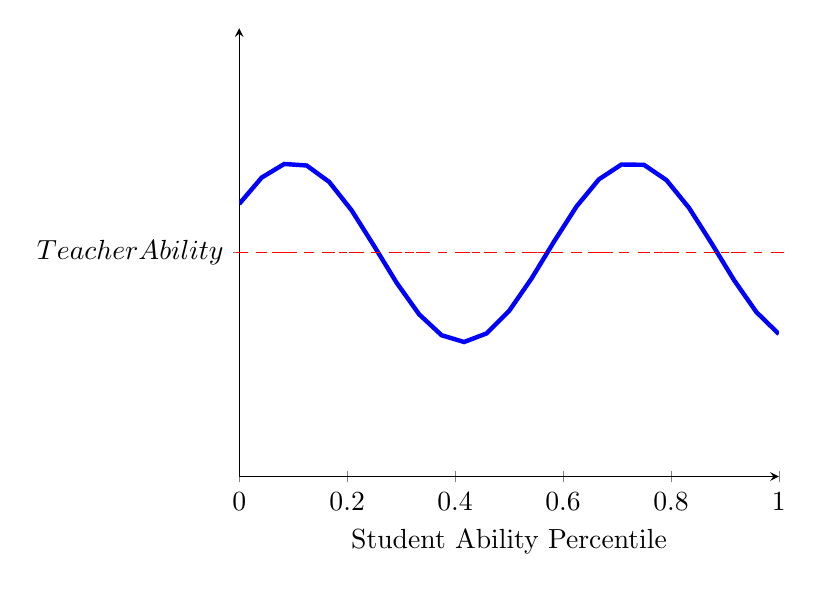
\begin{tikzpicture}
    \begin{axis}[ymin=0.25, ymax=0.75, ytick={0.5}, yticklabel=$TeacherAbility$, axis x line=bottom, axis y line=left, xlabel = Student Ability Percentile]
        \addplot[domain=0:1, blue, ultra thick] {.5 + .1*cos(deg(10*(x - .1)))};
        \addplot[domain=0:1, mark=-, red, dashed] {0.5};
    \end{axis}
\end{tikzpicture}



\end{document}